\section{What the Graphs Claim vs.\ What the Model Does}
\paragraph{The shortcuts are in the replacement, not the model.} Is the shallow graph a faithful picture of a model that takes logit-level shortcuts? Certification only checks the sign of the logit. We therefore measure $r_\mathrm{bypass}$: the mean $|\Delta\mathrm{logit}|$ when the upstream inputs and earlier sites are swapped while site $k$ is kept, relative to swapping site $k$ itself. In the original models $r_\mathrm{bypass}=\RbypassAllOrig$ on average, and the bypass swap never flips a decision. The \emph{replacement} models running the same test are far less bypass-free: $r_\mathrm{bypass}=\RbypassAllPLT$ for PLT and $\RbypassAllCLT$ for CLT, reaching $\RbypassPLTDThree$ and $\RbypassCLTDThree$ at $D=3$ (against $\RbypassOrigDThree$ for the original; not measured at $D=4$). They even flip up to $\BypassFlipMaxCLT$ of decisions. The CLT bypasses more than the PLT in $\NHopsCLTgtPLT$ of $\NHopsTotal$ (model, hop) pairs (Table~\ref{tab:bypass}). Accurate reconstruction on the data distribution therefore does not constrain counterfactual behaviour, and the depth the graph loses is introduced by the transcoders.
\begin{table}[t]\centering\caption{Logit-level bypass ratio $r_\mathrm{bypass}$ (lower = more faithful to the stepwise circuit).}\label{tab:bypass}\begin{tabular}{rrrr}\toprule
$D$ & original & PLT & CLT\\\midrule
2 & 0.060 & 0.107 & 0.108\\
3 & 0.042 & 0.148 & 0.321\\
\bottomrule\end{tabular}
\end{table}
\paragraph{Route freezing.} Freezing the CLT's cross-layer decoder writes at their base values leaves counterfactual accuracy at $\StepOnlyCLTDThree$ ($D=3$) and $\StepOnlyCLTDFour$ ($D=4$). Allowing \emph{only} the skip writes to update gives $\SkipOnlyCLTDFour$. The CLT's extra bypass therefore lives mostly in encoders that read upstream residual directions, not in its skip decoders.
\paragraph{How well the linearised graph predicts ablations.} The graph-predicted logit change from ablating a feature correlates with the actual change at $r=\AblRPLT$ for PLT but only $r=\AblRCLT$ for CLT (Fig.~\ref{fig:val}). CLT graphs are less faithful to their own replacement model.
\paragraph{Decodable is not causally used.} At the designated site, $\NAtSiteBoth$/$\NAtSite$ (point, hop) pairs are both decodable and causal. After the site, $\NAfterDecodable$ pairs are decodable and $\NAfterCausal$ are causal. \emph{Before} the hop is computed, $\NBeforeDecodable$ pairs are already decodable, because an AND of available inputs is linearly separable, yet $\NBeforeDecodableCausal$ are causal (1000-permutation probes; smallest $p=\MinPermP$).
\begin{figure}[t]\centering
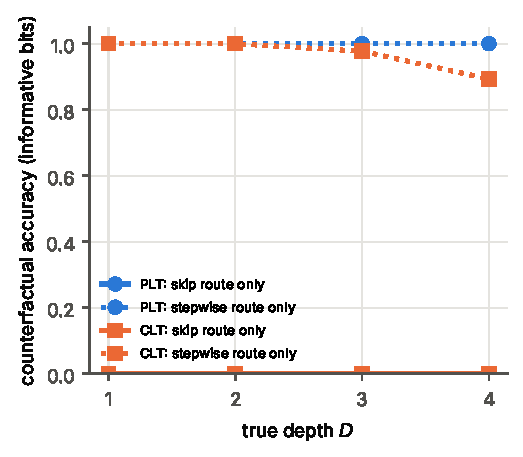
\includegraphics[width=0.48\linewidth]{figures/fig4_skip_dependence.pdf}\hfill
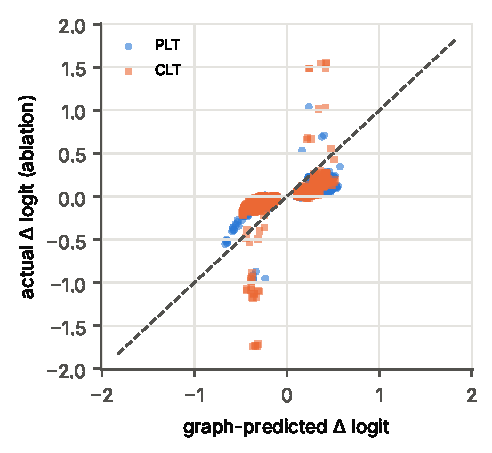
\includegraphics[width=0.44\linewidth]{figures/fig5_ablation_check.pdf}
\caption{Left: counterfactual accuracy when only the skip route or only the stepwise route may update. Right: graph-predicted vs.\ actual effect of ablating a feature.}\label{fig:val}\end{figure}
